\ifx\wholebook\relax \else
% ------------------------

% \documentclass[UTF8]{ctexart}
\documentclass[UTF8]{article}

%%
% loading packages
%
\newif\ifpdf
\ifx\pdfoutput\undefined % We're not running pdftex
  \pdffalse
\else
  \pdftrue
\fi
%
%
\ifpdf
  \RequirePackage[pdftex,%
            CJKbookmarks,%
       bookmarksnumbered,%
              colorlinks,%
          linkcolor=blue,%
              hyperindex,%
        plainpages=false,%
       pdfstartview=FitH]{hyperref}
\else
  \RequirePackage[dvipdfm,%
             CJKbookmarks,%
        bookmarksnumbered,%
               colorlinks,%
           linkcolor=blue,%
               hyperindex,%
         plainpages=false,%
        pdfstartview=FitH]{hyperref}
  \AtBeginDvi{\special{pdf:tounicode GBK-EUC-UCS2}} % GBK -> Unicode
\fi
\usepackage{hyperref}

% other packages
%-----------------------------------------------------------------------------
\usepackage{graphicx, color}
\usepackage{CJK}
%
% for programming 
%
\usepackage{verbatim}
\usepackage{listings}


\lstdefinelanguage{Smalltalk}{
  morekeywords={self,super,true,false,nil,thisContext}, % This is overkill
  morestring=[d]',
  morecomment=[s]{"}{"},
  alsoletter={\#:},
  escapechar={!},
  literate=
    {BANG}{!}1
    {UNDERSCORE}{\_}1
    {\\st}{Smalltalk}9 % convenience -- in case \st occurs in code
    % {'}{{\textquotesingle}}1 % replaced by upquote=true in \lstset
    {_}{{$\leftarrow$}}1
    {>>>}{{\sep}}1
    {^}{{$\uparrow$}}1
    {~}{{$\sim$}}1
    {-}{{\sf -\hspace{-0.13em}-}}1  % the goal is to make - the same width as +
    %{+}{\raisebox{0.08ex}{+}}1		% and to raise + off the baseline to match -
    {-->}{{\quad$\longrightarrow$\quad}}3
	, % Don't forget the comma at the end!
  tabsize=2
}[keywords,comments,strings]

\lstloadlanguages{C++, Lisp, Smalltalk}

% ======================================================================

\def\BibTeX{{\rm B\kern-.05em{\sc i\kern-.025em b}\kern-.08em
    T\kern-.1667em\lower.7ex\hbox{E}\kern-.125emX}}

\newtheorem{theorem}{Theorem}

%
% mathematics
%
\newcommand{\be}{\begin{equation}}
\newcommand{\ee}{\end{equation}}
\newcommand{\bmat}[1]{\left( \begin{array}{#1} }
\newcommand{\emat}{\end{array} \right) }
\newcommand{\VEC}[1]{\mbox{\boldmath $#1$}}

% numbered equation array
\newcommand{\bea}{\begin{eqnarray}}
\newcommand{\eea}{\end{eqnarray}}

% equation array not numbered
\newcommand{\bean}{\begin{eqnarray*}}
\newcommand{\eean}{\end{eqnarray*}}

\RequirePackage{CJK,CJKnumb,CJKulem,CJKpunct}
% we use CJK as default environment
\AtBeginDocument{\begin{CJK*}{GBK}{song}\CJKtilde\CJKindent\CJKcaption{GB}}
\AtEndDocument{\clearpage\end{CJK*}}

%
% loading packages
%

\RequirePackage{ifpdf}
\RequirePackage{ifxetex}

%
%
\ifpdf
  \RequirePackage[pdftex,%
       bookmarksnumbered,%
              colorlinks,%
          linkcolor=blue,%
              hyperindex,%
        plainpages=false,%
       pdfstartview=FitH]{hyperref}
\else\ifxetex
  \RequirePackage[bookmarksnumbered,%
               colorlinks,%
           linkcolor=blue,%
               hyperindex,%
         plainpages=false,%
        pdfstartview=FitH]{hyperref}
\else
  \RequirePackage[dvipdfm,%
        bookmarksnumbered,%
               colorlinks,%
           linkcolor=blue,%
               hyperindex,%
         plainpages=false,%
        pdfstartview=FitH]{hyperref}
\fi\fi
%\usepackage{hyperref}

% other packages
%--------------------------------------------------------------------------
\usepackage{graphicx, color}
\usepackage{subfig}
\usepackage{tikz}
\usetikzlibrary{matrix,positioning}

\usepackage{amsmath, amsthm, amssymb} % for math
\usepackage{exercise} % for exercise
\usepackage{import} % for nested input

%
% for programming
%
\usepackage{verbatim}
\usepackage{listings}
%\usepackage{algorithmic} %old version; we can use algorithmicx instead
\usepackage{algorithm}
\usepackage[noend]{algpseudocode} %for pseudo code, include algorithmicsx automatically
\usepackage{appendix}
\usepackage{makeidx} % for index support
\usepackage{titlesec}

\usepackage[cm-default]{fontspec}
\usepackage{xunicode}

% detect and select Chinese font
% ------------------------------
% the following cmd can list all availabe Chinese fonts in host.
% fc-list :lang=zh
\def\myfont{STHeiti}  % Under Mac OS X
\def\linuxfallback{WenQuanYi Micro Hei} % Under Linux
\def\winfallback{SimSun} % Under Windows
\suppressfontnotfounderror1 % Avoid setting exit code (error level) to break make process
\count255=\interactionmode
\batchmode
\font\foo="\myfont"\space at 10pt
\ifx\foo\nullfont
  \font\foo = "\linuxfallback"\space at 10pt
  \ifx\foo\nullfont
    \font\foo = "\winfallback"\space at 10pt
    \ifx\foo\nullfont
      \errorstopmode
      \errmessage{no suitable Chinese font found}
    \else
      \let\myfont=\winfallback % Windows
    \fi
  \else
    \let\myfont=\linuxfallback % Linux
  \fi
\fi
\interactionmode=\count255
\setmainfont[Mapping=tex-text]{\myfont}

\XeTeXlinebreaklocale "zh"  % to solve the line breaking issue
\XeTeXlinebreakskip = 0pt plus 1pt minus 0.1pt

\titleformat{\paragraph}
{\normalfont\normalsize\bfseries}{\theparagraph}{1em}{}
\titlespacing*{\paragraph}
{0pt}{3.25ex plus 1ex minus .2ex}{1.5ex plus .2ex}

\lstdefinelanguage{Smalltalk}{
  morekeywords={self,super,true,false,nil,thisContext}, % This is overkill
  morestring=[d]',
  morecomment=[s]{"}{"},
  alsoletter={\#:},
  escapechar={!},
  literate=
    {BANG}{!}1
    {UNDERSCORE}{\_}1
    {\\st}{Smalltalk}9 % convenience -- in case \st occurs in code
    % {'}{{\textquotesingle}}1 % replaced by upquote=true in \lstset
    {_}{{$\leftarrow$}}1
    {>>>}{{\sep}}1
    {^}{{$\uparrow$}}1
    {~}{{$\sim$}}1
    {-}{{\sf -\hspace{-0.13em}-}}1  % the goal is to make - the same width as +
    %{+}{\raisebox{0.08ex}{+}}1		% and to raise + off the baseline to match -
    {-->}{{\quad$\longrightarrow$\quad}}3
	, % Don't forget the comma at the end!
  tabsize=2
}[keywords,comments,strings]

% for better Haskell code outlook
\lstdefinelanguage{Haskell}{
  basicstyle=\small\ttfamily,
  flexiblecolumns=false,
  basewidth={0.5em,0.45em},
  literate={+}{{$+$}}1 {/}{{$/$}}1 {*}{{$*$}}1 {=}{{$=$}}1
           {>}{{$>$}}1 {<}{{$<$}}1 {\\}{{$\lambda$}}1
           {\\\\}{{\char`\\\char`\\}}1
           {->}{{$\rightarrow$}}2 {>=}{{$\geq$}}2 {<-}{{$\leftarrow$}}2
           {<=}{{$\leq$}}2 {=>}{{$\Rightarrow$}}2
           {\ .}{{$\circ$}}2 {\ .\ }{{$\circ$}}2
           {>>}{{>>}}2 {>>=}{{>>=}}2
           {|}{{$\mid$}}1
}[keywords,comments,strings]

\lstloadlanguages{C, C++, Lisp, Haskell, Python, Smalltalk}

\lstset{
  showstringspaces = false
}

% ======================================================================

\def\BibTeX{{\rm B\kern-.05em{\sc i\kern-.025em b}\kern-.08em
    T\kern-.1667em\lower.7ex\hbox{E}\kern-.125emX}}

%
% mathematics
%
\newcommand{\be}{\begin{equation}}
\newcommand{\ee}{\end{equation}}
\newcommand{\bmat}[1]{\left( \begin{array}{#1} }
\newcommand{\emat}{\end{array} \right) }
\newcommand{\VEC}[1]{\mbox{\boldmath $#1$}}

% numbered equation array
\newcommand{\bea}{\begin{eqnarray}}
\newcommand{\eea}{\end{eqnarray}}

% equation array not numbered
\newcommand{\bean}{\begin{eqnarray*}}
\newcommand{\eean}{\end{eqnarray*}}

\newtheorem{theorem}{Theorem}[section]
\newtheorem{lemma}[theorem]{Lemma}
\newtheorem{proposition}[theorem]{Proposition}
\newtheorem{corollary}[theorem]{Corollary}


\setcounter{page}{1}

\begin{document}

%--------------------------

% ================================================================
%                 COVER PAGE
% ================================================================

\title{前言}

\author{刘新宇
\thanks{{\bfseries 刘新宇} \newline
  Email: liuxinyu95@gmail.com \newline}
  }

\maketitle
\fi

\markboth{前言}{初等算法}

% ================================================================
%                 Why
% ================================================================
\section{Why?}
\label{why}

“算法有用么?”经常有人问我这个问题。很多人在工作中根本不用算法。偶尔碰到的时候,也不过是使用一些实现好的库。例如C++标准模版库STL中有现成的排序、查找函数;常用的数据结构如向量(vector)、队列(queue)、集合(set)也都实现好了。日常工作中了解如何使用这些库似乎就足够了。

算法在解决一些“有趣”的问题时,会扮演关键角色。但是这些问题本身的价值,却是仁者见仁、智者见智。

让我们用例子来说话吧。下面两道题目,即使是初学编程的新手,似乎也很容易解决。

% ================================================================
%      Mininum free ID problem. The power of algorithms
% ================================================================
\section{最小可用ID,算法的威力}
\label{min-free} \index{minimum free number}

这道题目来自Richard Bird书中的第一章\cite{Bird-book}。现代社会中,有很多服务依赖一种被称为ID的概念。例如身份证就是一种ID,银行账户也是一种ID,电话号码本质上也是一种ID。假设我们使用非负整数作为某个系统的的ID,所有用户都由一个ID唯一确定。任何时间,这个系统中有些ID处在使用中的状态,有些ID则可以用于分配给新用户。现在的问题是,怎样才能找到最小的可用ID呢?例如下面的列表记录了当前正在被使用的ID:

\begin{verbatim}
[18, 4, 8, 9, 16, 1, 14, 7, 19, 3, 0, 5, 2, 11, 6]
\end{verbatim}

最小可用的ID,也就是不在这个列表中的最小整数是10。这个题目看上去是如此简单,我们可以立即写出下面解法:

\begin{algorithmic}[1]
\Function{Min-Free}{$A$}
  \State $x \gets 0$
  \Loop
    \If{$x \notin A$}
      \State \Return $x$
    \Else
      \State $x \gets x + 1$
    \EndIf
  \EndLoop
\EndFunction
\end{algorithmic}

其中符号$\notin$的实现如下:

\begin{algorithmic}[1]
\Function{`$\notin$'}{$x, X$}
  \For{$i \gets 1 $ to $|X|$}
    \If{$x = X[i]$}
      \State \Return False
    \EndIf
  \EndFor
  \State \Return True
\EndFunction
\end{algorithmic}

有些编程语言内置了这一线性查找的实现。例如我们可以直接将这一解法翻译成下面的Python程序。

\lstset{language=Python}
\begin{lstlisting}
def brute_force(lst):
    i = 0
    while True:
        if i not in lst:
            return i
        i = i + 1
\end{lstlisting}

但是这道题目仅仅是看上去简单。在一个存储了几百万个ID的大型系统中,这个方法的的性能很差。对于一个长度为n的ID列表,它需要$O(n^2)$的时间才能找到最小可用的ID。在我的计算机上(双核2.10GHz处理器,2G内存),使用这一方法的C语言程序平均需要约5.4秒才能在十万个ID中找到答案\footnote{所有代码均可随本书一起下载}。当ID的数量上升到一百万时,平均用时则长达8分钟。

\subsection{改进一}
改进这一解法的关键基于这一事实:对于任何$n$个非负整数$x_1, x_2, ..., x_n$,如果存在小于$n$的可用整数,必然存在某个$x_i$不在$[0, n)$这个范围内。否则这些整数一定是$0, 1, ..., n-1$的某个排列,这种情况下,最小的可用整数是$n$。于是我们有如下结论:

\be
minfree(x_1, x_2, ..., x_n) \leq n
\label{min-free}
\ee

根据这一结论,我们可以用一个长度为$n+1$的数组,来标记区间$[0, n]$内的某个整数是否可用。

\begin{algorithmic}[1]
\Function{Min-Free}{$A$}
  \State $F \gets [False, False, ..., False]$ where $|F| = n+1$
  \For{$\forall x \in A$}
    \If{$x < n$}
      \State $F[x] \gets$ True
    \EndIf
  \EndFor
  \For{$i \gets [0, n]$}
    \If{$F[i] =$ False}
      \State \Return $i$
    \EndIf
  \EndFor
\EndFunction
\end{algorithmic}

其中第2行将标志数组中的所有值初始化为False,这一步骤需要$O(n)$的时间。接着我们遍历$A$中的所有元素,只要小于$n$,就将相应的标记置为True。这一过程也需要$O(n)$的时间。最后我们再线性查找标志数组中第一个值为Fasle的位置。整个算法的性能是线性时间$O(n)$的。注意,我们使用了$n+1$个标志,而不是$n$个标志。这样无需额外处理,就可以应对$sorted(A) = [0, 1, 2, ..., n-1]$
的特殊情况。

虽然这个方法只需要线性时间,但是它需要使用$O(n)$的空间来存储标志。

这一方法比之前的暴力解法快很多。在我的计算机上,相应的Python程序平均只用0.02秒,就可以在十万个整数中找到答案。

我们还可以继续优化。每次查找,我们都需要申请长度为$n+1$的数组;查找结束后,这个数组又被释放掉了。反复的申请和释放会占用不少时间。我们可以预先准备好足够长的数组,然后每次查找都复用它。另外,我们可以使用二进制的位来保存标志,这样能节约不少空间。下面的C语言程序实现了这两点小改进。

\lstset{language = C}
\begin{lstlisting}
#define N 1000000 // 1 million
#define WORD_LENGTH sizeof(int) * 8

void setbit(unsigned int* bits, unsigned int i){
  bits[i / WORD_LENGTH] |= 1<<(i % WORD_LENGTH);
}

int testbit(unsigned int* bits, unsigned int i){
  return bits[i/WORD_LENGTH] & (1<<(i % WORD_LENGTH));
}

unsigned int bits[N/WORD_LENGTH+1];

int min_free(int* xs, int n){
  int i, len = N/WORD_LENGTH+1;
  for(i=0; i<len; ++i)
    bits[i]=0;
  for(i=0; i<n; ++i)
    if(xs[i]<n)
      setbit(bits, xs[i]);
  for(i=0; i<=n; ++i)
    if(!testbit(bits, i))
      return i;
}
\end{lstlisting}

在我的计算机上,这段C程序处理一百万个整数,平均用时仅仅0.023秒。最后一个for循环还能
进一步改进如下,但这些都是一些微调了。

\begin{lstlisting}
  for(i=0; ; ++i)
    if(~bits[i] !=0 )
      for(j=0; ; ++j)
	if(!testbit(bits, i*WORD_LENGTH+j))
	  return i*WORD_LENGTH+j;
\end{lstlisting}

\subsection{改进二、分而治之}
我们在速度上的改进是以空间上的消耗为代价的。由于维护了一个长度为$n$的标志数组,当$n$很大时,空间上的性能就成了新的瓶颈。

分而治之的典型策略是将问题分解为若干较小规模的子问题,然后逐步解决这些子问题以得到最终的结果。

我们可以将所有满足$x_i \leq \lfloor n/2 \rfloor$的整数放入一个子序列$A'$;将剩余的其他整数放入另外一个序列$A''$。根据公式\ref{min-free},如果序列$A'$的长度正好是$\lfloor n/2 \rfloor$,这说明前一半的整数已经“满了”,最小的可用整数一定可以在$A''$中递归地找到。否则,最小的可用整数可以在$A'$中找到。总之,通过这一划分,问题的规模减小了。

需要注意的是,当我们在子序列$A''$中递归查找时,边界情况发生了一些变化,我们不再是从0开始寻找最小可用整数,查找的下界变成了$\lfloor n/2 \rfloor + 1$。因此我们的算法应定义为$minfree(A, l, u)$,其中$l$和$u$分别是上下界。

递归结束的边界条件是当待查找的序列变为空的时候,此时我们只需要返回下界作为结果即可。

根据上述思路,分而治之的解法可以形式化地定义为一个函数:

\[
minfree(A) = search(A, 0, |A|-1)
\]

\[
search(A, l, u) = \left \{
       \begin{array}
       {r@{\quad:\quad}l}
       l & A = \phi \\
       search(A'', m+1, u) &  |A'| = m - l + 1 \\
       search(A',  l, m) & otherwise
       \end{array}
\right.
\]

其中

\[ \begin{array}{l}
m = \displaystyle \lfloor \frac{l+u}{2} \rfloor \\
A'  = \{ \forall x \in A \wedge x \leq m \} \\
A'' = \{ \forall x \in A \wedge x > m \} \\
\end{array} \]

这一方法并不需要额外的空间\footnote{有人认为需要$O(\lg n)$的栈空间来做递归调用的book-keeping。我们稍后会看到,这一调用实际上是尾递归,有些编译器,例如gcc可以通过-O2选项消除递归。我们也可以手工将递归转换为迭代。}。每次调用需要进行$O(|A|)$次比较来划分出子序列$A'$和$A''$。之后,问题的规模减半,所以这个算法用时为$T(n) = T(n/2) + O(n)$,化简可知其结果为$O(n)$。另外,我们也可以这样分析其复杂度:第一次需要$O(n)$次比较来划分子序列$A'$和$A''$,第二次仅需要比较$O(n/2)$次,第三次需要比较$O(n/4)$次……总时间为$O(n + n/2 + n/4 + ...) = O(2n) = O(n)$。

在有些函数式编程语言,例如Haskell中,划分一个序列已经被作为库函数提供了。下面的例子代码实现了分而治之的算法。

\lstset{language=Haskell}
\begin{lstlisting}
import Data.List

minFree xs = bsearch xs 0 (length xs - 1)

bsearch xs l u | xs == [] = l
               | length as == m - l + 1 = bsearch bs (m+1) u
               | otherwise = bsearch as l m
    where
      m = (l + u) `div` 2
      (as, bs) = partition (<=m) xs
\end{lstlisting}

\subsection{简洁与性能——鱼和熊掌}
使用imperative编程语言的读者可能会担心这种实现的性能。对于最小可用ID问题,递归
Imperative language programmers may be concerned about the performance
of this kind of implementation. For instance in this minimum
free ID problem, the number of recursive calls is in $O(\lg n)$
, which means the stack size consumed is in $O(\lg n)$.
It's not free in terms of space. But if we want to avoid that
, we can eliminate the recursion by replacing it by an iteration
\footnote{This is done automatically in most functional languages
since our function is in tail recursive form which lends itself
perfectly to this transformation} which yields the following C program.

\lstset{language=C}
\begin{lstlisting}
int min_free(int* xs, int n){
  int l=0;
  int u=n-1;
  while(n){
    int m = (l + u) / 2;
    int right, left = 0;
    for(right = 0; right < n; ++ right)
      if(xs[right] <= m){
	swap(xs[left], xs[right]);
	++left;
      }
    if(left == m - l + 1){
      xs = xs + left;
      n  = n - left;
      l  = m+1;
    }
    else{
      n = left;
      u = m;
    }
  }
  return l;
}
\end{lstlisting}

This program uses a `quick-sort' like approach to re-arrange the
array so that all the elements before $left$ are less than or equal
to $m$; while those between $left$ and $right$ are greater
than $m$. This is shown in figure \ref{fig:divide}.

\begin{figure}[htbp]
  \centering
  \includegraphics[scale=1]{img/divide-by-m.ps}
  \caption{Divide the array, all $x[i] \leq m$ where $0 \leq i < left$; while all $x[i] > m$ where $left \leq i < right$. The left elements are unknown.} \label{fig:divide}
\end{figure}

This program is fast and it doesn't need extra stack space. However,
compared to the previous Haskell program, it's hard to read and the
expressiveness decreased. We have to balance performance
and expressiveness.

\section{The number puzzle, power of data structure}

If the first problem, to find the minimum free number, is a some what
useful in practice, this problem is a `pure' one for fun. The puzzle
is to find the 1,500th number, which only contains factor 2, 3 or 5.
The first 3 numbers are of course 2, 3, and 5. Number $60 = 2^23^15^1$,
However it is the 25th number. Number $21 = 2^03^17^1$, isn't a valid
number because it contains a factor 7. The first 10 such numbers are list
as the following.

2,3,4,5,6,8,9,10,12,15

If we consider $1=2^03^05^0$, then 1 is also a valid number and it is
the first one.

\subsection{The brute-force solution}
It seems the solution is quite easy without need any serious algorithms.
We can check all numbers from 1, then extract all factors of 2, 3 and 5
to see if the left part is 1.

\begin{algorithmic}[1]
\Function{Get-Number}{$n$}
  \State $x \gets 1$
  \State $i \gets 0$
  \Loop
    \If{\Call{Valid?}{$x$}}
      \State $i \gets i + 1$
      \If{$i = n$}
        \State \Return $x$
      \EndIf
    \EndIf
    \State $x \gets x + 1$
  \EndLoop
\EndFunction
\Statex
\Function{Valid?}{$x$}
  \While{$x \bmod 2 = 0$}
    \State $x \gets x / 2$
  \EndWhile
  \While{$x \bmod 3 = 0$}
    \State $x \gets x / 3$
  \EndWhile
  \While{$x \bmod 5 = 0$}
    \State $x \gets x / 5$
  \EndWhile
  \If{$x = 1$}
    \State \Return $True$
  \Else
    \State \Return $False$
  \EndIf
\EndFunction
\end{algorithmic}

This `brute-force' algorithm works for most small $n$. However, to find
the 1500th number (which is 859963392), the C program based on this
algorithm takes 40.39 seconds in my computer. I have to kill the program
after 10 minutes when I increased $n$ to 15,000.

\subsection{Improvement 1}
Analysis of the above algorithm shows that modular and divide calculations
are very expensive \cite{Bentley}. And they executed a lot in loops.
Instead of checking a number contains only 2, 3, or 5 as factors, one
alternative solution is to construct such number by these factors.

We start from 1, and times it with 2, or 3, or 5 to generate rest numbers.
The problem turns to be how to generate the candidate number in order?
One handy way is to utilize the queue data structure.

A queue data structure is used to push elements at one end, and pops
them at the other end. So that the element be pushed first is also
be popped out first. This property is called FIFO (First-In-First-Out).

The idea is to push 1 as the only element to the queue, then we pop
an element, times it with 2, 3, and 5, to get 3 new elements. We
then push them back to the queue in order. Note that, the new elements may
have already existed in the queue. In such case, we just drop the
element. The new element may also smaller than the others in the queue,
so we must put them to the correct position. Figure \ref{fig:queues}
illustrates this idea.

\begin{figure}[htbp]
       \begin{center}
       	  \includegraphics[scale=0.5]{img/q1.ps}
       	  \includegraphics[scale=0.5]{img/q2.ps}
       	  \includegraphics[scale=0.5]{img/q3.ps}
       	  \includegraphics[scale=0.5]{img/q4.ps}
        \caption{First 4 steps of constructing numbers with a queue. \newline
        1. Queue is initialized with 1 as the only element;\newline
        2. New elements 2, 3, and 5 are pushed back; \newline
        3. New elements 4, 6, and 10, are pushed back in order; \newline
        4. New elements 9 and 15 are pushed back, element 6 already exists.} \label{fig:queues}
       \end{center}
\end{figure}

This algorithm is shown as the following.

\begin{algorithmic}[1]
\Function{Get-Number}{$n$}
  \State $Q \gets NIL$
  \State \Call{Enqueue}{$Q, 1$}
  \While{$n > 0$}
    \State $x \gets$ \Call{Dequeue}{$Q$}
    \State \Call{Unique-Enqueue}{$Q, 2x$}
    \State \Call{Unique-Enqueue}{$Q, 3x$}
    \State \Call{Unique-Enqueue}{$Q, 5x$}
    \State $n \gets n-1$
  \EndWhile
  \State \Return $x$
\EndFunction
\Statex
\Function{Unique-Enqueue}{$Q, x$}
  \State $i \gets 0$
  \While{$i < |Q| \wedge Q[i] < x$}
    \State $i \gets i + 1$
  \EndWhile
  \If{$i < |Q| \wedge x = Q[i]$}
    \State \Return
  \EndIf
  \State \Call{Insert}{$Q, i, x$}
\EndFunction
\end{algorithmic}

The insert function takes $O(|Q|)$ time to find the proper position and insert
it. If the element has already existed, it just returns.

A rough estimation tells that the length of the queue increase proportion to $n$,
(Each time, we extract one element, and pushed 3 new, the increase ratio $\leq$ 2),
so the total running time is $O(1+2+3+...+n) = O(n^2)$.

Figure\ref{fig:big-O-1q} shows the number of queue access time against $n$.
It is quadratic curve which reflect the $O(n^2)$ performance.

\begin{figure}[htbp]
       \begin{center}
       	  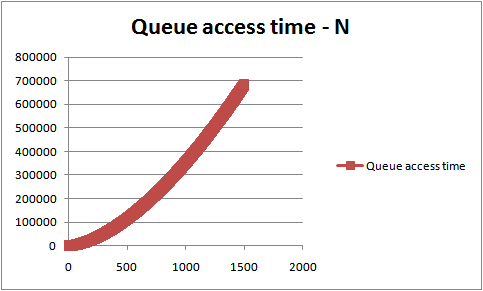
\includegraphics[scale=0.5]{img/big-O-1q.eps}
        \caption{Queue access count v.s. $n$.} \label{fig:big-O-1q}
       \end{center}
\end{figure}

The C program based on this algorithm takes only 0.016[s] to get the right answer
859963392. Which is 2500 times faster than the brute force solution.

%% Functional 1Q solution
Improvement 1 can also be considered in recursive way. Suppose $X$ is the infinity
series for all numbers which only contain factors of 2, 3, or 5. The following
formula shows an interesting relationship.

\be
  X = \{1\} \cup \{2x: \forall x \in X\} \cup \{3x: \forall x \in X \} \cup \{5x: \forall x \in X \}
\ee

Where we can define $\cup$ to a special form so that all elements are stored in order
as well as unique to each other. Suppose that $X=\{x_1, x_2, x_3...\}$, $Y=\{y_1, y_2, y_3, ...\}$, $X' = \{x_2, x_3, ...\}$ and $Y'=\{y_2, y_3, ...\}$. We have

\[
X \cup Y = \left \{
  \begin{array}{r@{\quad:\quad}l}
  X & Y = \phi \\
  Y & X = \phi \\
  \{ x_1, X' \cup Y \} & x_1 < y_1 \\
  \{ x_1, X' \cup Y' \} & x_1 = y_1 \\
  \{ y_1, X \cup Y' \} & x_1 > y_1
  \end{array}
\right.
\]

In a functional programming language such as Haskell, which supports
lazy evaluation, The above infinity series functions can be translate
into the following program.

\lstset{language=Haskell}
\begin{lstlisting}
ns = 1:merge (map (*2) ns) (merge (map (*3) ns) (map (*5) ns))

merge [] l = l
merge l [] = l
merge (x:xs) (y:ys) | x <y = x : merge xs (y:ys)
                    | x ==y = x : merge xs ys
                    | otherwise = y : merge (x:xs) ys
\end{lstlisting}

By evaluate ns !! (n-1), we can get the 1500th number as
below.

\begin{verbatim}
>ns !! (1500-1)
859963392
\end{verbatim}

\subsection{Improvement 2}
Considering the above solution, although it is much faster than the brute-force one,
It still has some drawbacks. It produces many duplicated numbers and they are
finally dropped when examine the queue. Secondly, it does linear scan and insertion
to keep the order of all elements in the queue, which degrade the ENQUEUE operation
from $O(1)$ to $O(|Q|)$.

If we use three queues instead of using only one, we can improve the solution one
step ahead. Denote these queues as $Q_2$, $Q_3$, and $Q_5$, and we initialize
them as $Q_2=\{ 2 \}$, $Q_3 = \{ 3\}$ and $Q_5 = \{ 5 \}$. Each time we DEQUEUEed
the smallest one from $Q_2$, $Q_3$, and $Q_5$ as $x$. And do the following test:

\begin{itemize}
\item If $x$ comes from $Q_2$, we ENQUEUE $2x$, $3x$, and $5x$ back to
$Q_2$, $Q_3$, and $Q_5$ respectively;
\item If $x$ comes from $Q_3$, we only need ENQUEUE $3x$ to $Q_3$, and $5x$ to $Q_5$;
We needn't ENQUEUE $2x$ to $Q_2$, because $2x$ have already existed in $Q_3$;
\item If $x$ comes from $Q_5$, we only need ENQUEUE $5x$ to $Q_5$; there is
no need to ENQUEUE $3x$, $5x$ to $Q_3$, $Q_5$ because they have already been
in the queues;
\end{itemize}

We repeatedly ENQUEUE the smallest one until we find the $n$-th element.

\begin{figure}[htbp]
       \begin{center}
       	  \includegraphics[scale=0.5]{img/q235-1.ps}
       	  \includegraphics[scale=0.5]{img/q235-2.ps}
       	  \includegraphics[scale=0.5]{img/q235-3.ps}
       	  \includegraphics[scale=0.5]{img/q235-4.ps}
        \caption{First 4 steps of constructing numbers with $Q_2$, $Q_3$, and $Q_5$. \newline
        1. Queues are initialized with 2, 3, 5 as the only element;\newline
        2. New elements 4, 6, and 10 are pushed back; \newline
        3. New elements 9, and 15, are pushed back; \newline
        4. New elements 8, 12, and 20 are pushed back; \newline
        5. New element 25 is pushed back.} \label{fig:q235}
       \end{center}
\end{figure}

The algorithm based on this idea is implemented as below.

\begin{algorithmic}[1]
\Function{Get-Number}{$n$}
  \If{$n = 1$}
    \State \Return $1$
  \Else
    \State $Q_2 \gets \{ 2 \}$
    \State $Q_3 \gets \{ 3 \}$
    \State $Q_5 \gets \{ 5 \}$
    \While{$n > 1$}
      \State $x \gets min($\Call{Head}{$Q_2$}, \Call{Head}{$Q_3$}, \Call{Head}{$Q_5$}$)$
      \If{$x = $ \Call{Head}{$Q_2$}}
        \State \Call{Dequeue}{$Q_2$}
        \State \Call{Enqueue}{$Q_2, 2x$}
        \State \Call{Enqueue}{$Q_3, 3x$}
        \State \Call{Enqueue}{$Q_5, 5x$}
      \ElsIf{$x=$ \Call{Head}{$Q_3$}}
        \State \Call{Dequeue}{$Q_3$}
        \State \Call{Enqueue}{$Q_3, 3x$}
        \State \Call{Enqueue}{$Q_5, 5x$}
      \Else
        \State \Call{Dequeue}{$Q_5$}
        \State \Call{Enqueue}{$Q_5, 5x$}
      \EndIf
      \State $n \gets n - 1$
    \EndWhile
    \State \Return $x$
  \EndIf
\EndFunction
\end{algorithmic}

This algorithm loops $n$ times, and within each loop, it extract one head
element from the three queues, which takes constant time. Then it appends
one to three new elements at the end of queues which bounds to constant time
too. So the total time of the algorithm bounds to $O(n)$. The C++ program
translated from this algorithm shown below takes less than 1 $\mu$s to
produce the 1500th number, 859963392.

\lstset{language=C++}
\begin{lstlisting}
typedef unsigned long Integer;

Integer get_number(int n){
  if(n==1)
    return 1;
  queue<Integer> Q2, Q3, Q5;
  Q2.push(2);
  Q3.push(3);
  Q5.push(5);
  Integer x;
  while(n-- > 1){
    x = min(min(Q2.front(), Q3.front()), Q5.front());
    if(x==Q2.front()){
      Q2.pop();
      Q2.push(x*2);
      Q3.push(x*3);
      Q5.push(x*5);
    }
    else if(x==Q3.front()){
      Q3.pop();
      Q3.push(x*3);
      Q5.push(x*5);
    }
    else{
      Q5.pop();
      Q5.push(x*5);
    }
  }
  return x;
}
\end{lstlisting}

This solution can be also implemented in Functional way. We define
a function $take(n)$, which will return the first $n$ numbers contains
only factor 2, 3, or 5.

\[
  take(n) = f(n, \{1\}, \{2\}, \{3\}, \{5\})
\]
Where
\[
 f(n, X, Q_2, Q_3, Q_5) = \left \{
  \begin{array}{r@{\quad:\quad}l}
  X & n = 1 \\
  f(n-1, X \cup \{x\}, Q_2', Q_3', Q_5') & otherwise
  \end{array}
\right.
\]

\[
 x = min(Q_{21}, Q_{31}, Q_{51})
\]
\[
 Q_2', Q_3', Q_5' = \left \{
 \begin{array}{r@{\quad:\quad}l}
 \{Q_{22}, Q_{23}, ...\} \cup \{2x\}, Q_3 \cup \{3x\}, Q_5 \cup \{5x\} & x = Q_{21} \\
 Q_2, \{Q_{32}, Q_{33}, ...\} \cup \{3x\}, Q5 \cup \{5x\} & x = Q_{31} \\
 Q_2, Q_3, \{Q_{52}, Q_{53}, ...\} \cup \{5x\} & x = Q_{51}
 \end{array}
 \right.
\]

And these functional definition can be realized in Haskell as the following.

\lstset{language=Haskell}
\begin{lstlisting}
ks 1 xs _ = xs
ks n xs (q2, q3, q5) = ks (n-1) (xs++[x]) update
    where
      x = minimum $ map head [q2, q3, q5]
      update | x == head q2 = ((tail q2)++[x*2], q3++[x*3], q5++[x*5])
             | x == head q3 = (q2, (tail q3)++[x*3], q5++[x*5])
             | otherwise = (q2, q3, (tail q5)++[x*5])

takeN n = ks n [1] ([2], [3], [5])
\end{lstlisting} %$

Invoke `last takeN 1500' will generate the correct answer 859963392.

% ================================================================
%                 Short summary
% ================================================================
\section{Notes and short summary}
If review the 2 puzzles, we found in both cases, the brute-force solutions
are so weak. In the first problem, it's quite poor in dealing with
long ID list, while in the second problem, it doesn't work at all.

The first problem shows the power of algorithms, while the second
problem tells why data structure is important. There are plenty
of interesting problems, which are hard to solve before computer
was invented. With the aid of computer and programming, we are able
to find the answer in a quite different way. Compare to what we
learned in mathematics course in school, we haven't been taught the method
like this.

While there have been already a lot of wonderful books about
algorithms, data structures and math, however, few of them
provide the comparison between the procedural solution and
the functional solution. From the above discussion, it can be
found that functional solution sometimes is very expressive
and they are close to what we are familiar in mathematics.

This series of post focus on providing both imperative and functional
algorithms and data structures. Many functional data structures
can be referenced from Okasaki's book\cite{okasaki-book}. While
the imperative ones can be founded in classic text books \cite{CLRS}
or even in WIKIpedia.
Multiple
programming languages, including, C, C++, Python, Haskell, and
Scheme/Lisp will be used. In order to make it easy to read
by programmers with different background, pseudo code and mathematical
function are the regular descriptions of each post.

The author is NOT a native English speaker, the reason why
this book is only available in English for the time being
is because the contents are still changing frequently. Any
feedback, comments, or criticizes are welcome.

\section{Structure of the contents}
In the following series of post, I'll first introduce about
elementary data structures before algorithms, because many
algorithms need knowledge of data structures as prerequisite.

The `hello world' data structure, binary search tree is the
first topic; Then we introduce how to solve the balance problem
of binary search tree. After that, I'll show other interesting
trees. Trie, Patricia, suffix trees are useful in text manipulation.
While B-trees are commonly used in file system and data base
implementation.

The second part of data structures is about heaps. We'll
provide a general Heap definition and introduce about binary
heaps by array and by explicit binary trees. Then we'll
extend to K-ary heaps including Binomial heaps, Fibonacci
heaps, and pairing heaps.

Array and queues are considered among the easiest data structures
typically, However, we'll show how difficult to implement
them in the third part.

As the elementary sort algorithms, we'll introduce insertion
sort, quick sort, merge sort etc in both imperative way
and functional way.

The final part is about searching, besides the element
searching, we'll also show string matching algorithms
such as KMP.

All the posts are provided under GNU FDL (Free document
license), and programs are under GNU GPL.

% ================================================================
%                 Appendix
% ================================================================
\section{Appendix} \label{appendix}
%\appendix
All programs provided along with this book are free for
downloading. download position:
  http://sites.google.com/site/algoxy/home

\begin{thebibliography}{99}

\bibitem{Bird-book}
Richard Bird. ``Pearls of functional algorithm design''. Cambridge University Press; 1 edition (November 1, 2010). ISBN-10: 0521513383

\bibitem{Bentley}
Jon Bentley. ``Programming Pearls(2nd Edition)''. Addison-Wesley Professional; 2 edition (October 7, 1999). ISBN-13: 978-0201657883

\bibitem{okasaki-book}
Chris Okasaki. ``Purely Functional Data Structures''. Cambridge university press, (July 1, 1999), ISBN-13: 978-0521663502

\bibitem{CLRS}
Thomas H. Cormen, Charles E. Leiserson, Ronald L. Rivest and Clifford Stein. ``Introduction to Algorithms, Second Edition''. The MIT Press, 2001. ISBN: 0262032937.

\end{thebibliography}

\ifx\wholebook\relax \else
\end{document}
\fi
